% !TeX spellcheck = pl_PL
%%%%%%%%%%%%%%%%%%%%%%%%%%%%%%%%%%%%%%%%%%%
%                                        %
% Szablon pracy dyplomowej inzynierskiej %
% zgodny  z aktualnymi  przepisami  SZJK %
%                                        %
%%%%%%%%%%%%%%%%%%%%%%%%%%%%%%%%%%%%%%%%%%
%                                        %
%  (c) Krzysztof Simiński, 2018-2023     %
%                                        %
%%%%%%%%%%%%%%%%%%%%%%%%%%%%%%%%%%%%%%%%%%
%                                        %
% Najnowsza wersja szablonów jest        %
% podstępna pod adresem                  %
% github.com/ksiminski/polsl-aei-theses  %
%                                        %
%%%%%%%%%%%%%%%%%%%%%%%%%%%%%%%%%%%%%%%%%%
%
%
% Projekt LaTeXowy zapewnia odpowiednie formatowanie pracy,
% zgodnie z wymaganiami Systemu zapewniania jakości kształcenia.
% Proszę nie zmieniać ustawień formatowania (np. fontu,
% marginesów, wytłuszczeń, kursywy itd. ).
%
% Projekt można kompilować na kilka sposobów.
%
% 1. kompilacja pdfLaTeX
%
% pdflatex main
% bibtex   main
% pdflatex main
% pdflatex main
%
%
% 2. kompilacja XeLaTeX
%
% Kompilatacja przy użyciu XeLaTeXa różni się tym, że na stronie
% tytułowej używany jest font Calibri. Wymaga to jego uprzedniego
% zainstalowania.
%
% xelatex main
% bibtex  main
% xelatex main
% xelatex main
%
%
%%%%%%%%%%%%%%%%%%%%%%%%%%%%%%%%%%%%%%%%%%%%%%%%%%%%%
% W przypadku pytań, uwag, proszę pisać na adres:   %
%      krzysztof.siminski(małpa)polsl.pl            %
%%%%%%%%%%%%%%%%%%%%%%%%%%%%%%%%%%%%%%%%%%%%%%%%%%%%%
%
% Chcemy ulepszać szablony LaTeXowe prac dyplomowych.
% Wypełniając ankietę spod poniższego adresu pomogą
% Państwo nam to zrobić. Ankieta jest całkowicie
% anonimowa. Dziękujemy!


% https://docs.google.com/forms/d/e/1FAIpQLScyllVxNKzKFHfILDfdbwC-jvT8YL0RSTFs-s27UGw9CKn-fQ/viewform?usp=sf_link
%
%%%%%%%%%%%%%%%%%%%%%%%%%%%%%%%%%%%%%%%%%%%%%%%%%%%%%%%%%%%%%%%%%%%%%%%%%

%%%%%%%%%%%%%%%%%%%%%%%%%%%%%%%%%%%%%%%%%%%%%%%
%                                             %
% PERSONALIZACJA PRACY – DANE PRACY           %
%                                             %
%%%%%%%%%%%%%%%%%%%%%%%%%%%%%%%%%%%%%%%%%%%%%%%

% Proszę wpisać swoje dane w poniższych definicjach.

% TODO
% dane autora
\newcommand{\FirstNameAuthor}{Piotr}
\newcommand{\SurnameAuthor}{Marcol}
\newcommand{\IdAuthor}{300463}   % numer albumu  (bez $\langle$ i $\rangle$)

% drugi autor:
%\newcommand{\FirstNameCoauthor}{Imię}   % Jeżeli jest drugi autor, to tutaj należy podać imię.
%\newcommand{\SurnameCoauthor}{Nazwisko} % Jeżeli jest drugi autor, to tutaj należy podać nazwisko.
%\newcommand{\IdCoauthor}{$\langle$wpisać właściwy$\rangle$}  % numer albumu drugiego autora (bez $\langle$ i $\rangle$)
% Gdy nie ma drugiego autora, należy zostawić poniższe definicje puste, jak poniżej. Gdy jest drugi autor, należy zakomentować te linie.
\newcommand{\FirstNameCoauthor}{} % Jeżeli praca ma tylko jednego autora, to dane drugiego autora zostają puste.
\newcommand{\SurnameCoauthor}{}   % Jeżeli praca ma tylko jednego autora, to dane drugiego autora zostają puste.
\newcommand{\IdCoauthor}{}  % Jeżeli praca ma tylko jednego autora, to dane drugiego autora zostają puste.
%%%%%%%%%%

\newcommand{\Supervisor}{Dr inż. Marcin Połomski}     % dane promotora (bez $\langle$ i $\rangle$)
\newcommand{\Title}{System zarządzania personelem}           % tytuł pracy po polsku
\newcommand{\TitleAlt}{Workforce management system}                     % thesis title in English
\newcommand{\Program}{Informatyka}            % kierunek studiów  (bez $\langle$ i $\rangle$)
\newcommand{\Specialisation}{Informatyczne Systemy Mobilne i Przemysłowe}     % specjalność  (bez $\langle$ i $\rangle$)
\newcommand{\Departament}{Katedra Algorytmiki i Oprogramowania}        % katedra promotora  (bez $\langle$ i $\rangle$)

% Jeżeli został wyznaczony promotor pomocniczy lub opiekun, proszę go/ją wpisać ...
% \newcommand{\Consultant}{$\langle$stopień naukowy imię i nazwisko$\rangle$} % dane promotora pomocniczego, opiekuna (bez $\langle$ i $\rangle$)
% ... w przeciwnym razie proszę zostawić puste miejsce jak poniżej:
\newcommand{\Consultant}{} % brak promotowa pomocniczego / opiekuna

% koniec fragmentu do modyfikacji
%%%%%%%%%%%%%%%%%%%%%%%%%%%%%%%%%%%%%%%%%%


%%%%%%%%%%%%%%%%%%%%%%%%%%%%%%%%%%%%%%%%%%%%%%%
%                                             %
% KONIEC PERSONALIZACJI PRACY                 %
%                                             %
%%%%%%%%%%%%%%%%%%%%%%%%%%%%%%%%%%%%%%%%%%%%%%%

%%%%%%%%%%%%%%%%%%%%%%%%%%%%%%%%%%%%%%%%


%%%%%%%%%%%%%%%%%%%%%%%%%%%%%%%%%%%%%%%%%%%%%%%
%                                             %
% PROSZĘ NIE MODYFIKOWAĆ PONIŻSZYCH USTAWIEŃ! %
%                                             %
%%%%%%%%%%%%%%%%%%%%%%%%%%%%%%%%%%%%%%%%%%%%%%%



\documentclass[a4paper,twoside,12pt]{book}
\usepackage[utf8]{inputenc}                                      
\usepackage[T1]{fontenc}  
\usepackage{amsmath,amsfonts,amssymb,amsthm}
\usepackage[british,polish]{babel} 
\usepackage{indentfirst}
\usepackage{xurl}
\usepackage{xstring}
\usepackage{ifthen}



\usepackage{ifxetex}

\ifxetex
	\usepackage{fontspec}
	\defaultfontfeatures{Mapping=tex—text} % to support TeX conventions like ``——-''
	\usepackage{xunicode} % Unicode support for LaTeX character names (accents, European chars, etc)
	\usepackage{xltxtra} % Extra customizations for XeLaTeX
\else
	\usepackage{lmodern}
\fi



\usepackage[margin=2.5cm]{geometry}
\usepackage{graphicx} 
\usepackage{hyperref}
\usepackage{booktabs}
\usepackage{tikz}
\usepackage{pgfplots}
\usepackage{mathtools}
\usepackage{geometry}
\usepackage{subcaption}   % subfigures
\usepackage[page]{appendix} % toc,
\renewcommand{\appendixtocname}{Dodatki}
\renewcommand{\appendixpagename}{Dodatki}
\renewcommand{\appendixname}{Dodatek}

\usepackage{csquotes}
\usepackage[natbib=true,backend=bibtex,maxbibnames=99]{biblatex}  % kompilacja bibliografii BibTeXem
%\usepackage[natbib=true,backend=biber,maxbibnames=99]{biblatex}  % kompilacja bibliografii Biberem
\bibliography{biblio/biblio}

\usepackage{ifmtarg}   % empty commands  

\usepackage{setspace}
\onehalfspacing


\frenchspacing



%%%% TODO LIST GENERATOR %%%%%%%%%

\usepackage{color}
\definecolor{brickred}      {cmyk}{0   , 0.89, 0.94, 0.28}

\makeatletter \newcommand \kslistofremarks{\section*{Uwagi} \@starttoc{rks}}
  \newcommand\l@uwagas[2]
    {\par\noindent \textbf{#2:} %\parbox{10cm}
{#1}\par} \makeatother


\newcommand{\ksremark}[1]{%
{%\marginpar{\textdbend}
{\color{brickred}{[#1]}}}%
\addcontentsline{rks}{uwagas}{\protect{#1}}%
}

\newcommand{\comma}{\ksremark{przecinek}}
\newcommand{\nocomma}{\ksremark{bez przecinka}}
\newcommand{\styl}{\ksremark{styl}}
\newcommand{\ortografia}{\ksremark{ortografia}}
\newcommand{\fleksja}{\ksremark{fleksja}}
\newcommand{\pauza}{\ksremark{pauza `--', nie dywiz `-'}}
\newcommand{\kolokwializm}{\ksremark{kolokwializm}}
\newcommand{\cudzyslowy}{\ksremark{,,polskie cudzysłowy''}}

%%%%%%%%%%%%%% END OF TODO LIST GENERATOR %%%%%%%%%%%

\newcommand{\printCoauthor}{%		
    \StrLen{\FirstNameCoauthor}[\FNCoALen]
    \ifthenelse{\FNCoALen > 0}%
    {%
		{\large\bfseries\Coauthor\par}
	
		{\normalsize\bfseries \LeftId: \IdCoauthor\par}
    }%
    {}
} 

%%%%%%%%%%%%%%%%%%%%%
\newcommand{\autor}{%		
    \StrLen{\FirstNameCoauthor}[\FNCoALenXX]
    \ifthenelse{\FNCoALenXX > 0}%
    {\FirstNameAuthor\ \SurnameAuthor, \FirstNameCoauthor\ \SurnameCoauthor}%
	{\FirstNameAuthor\ \SurnameAuthor}%
}
%%%%%%%%%%%%%%%%%%%%%

\StrLen{\FirstNameCoauthor}[\FNCoALen]
\ifthenelse{\FNCoALen > 0}%
{%
\author{\FirstNameAuthor\ \SurnameAuthor, \FirstNameCoauthor\ \SurnameCoauthor}
}%
{%
\author{\FirstNameAuthor\ \SurnameAuthor}
}%

%%%%%%%%%%%% ZYWA PAGINA %%%%%%%%%%%%%%%
% brak kapitalizacji zywej paginy
\usepackage{fancyhdr}
\pagestyle{fancy}
\fancyhf{}
\fancyhead[LO]{\nouppercase{\it\rightmark}}
\fancyhead[RE]{\nouppercase{\it\leftmark}}
\fancyhead[LE,RO]{\it\thepage}


\fancypagestyle{tylkoNumeryStron}{%
   \fancyhf{} 
   \fancyhead[LE,RO]{\it\thepage}
}

\fancypagestyle{bezNumeracji}{%
   \fancyhf{} 
   \fancyhead[LE,RO]{}
}


\fancypagestyle{NumeryStronNazwyRozdzialow}{%
   \fancyhf{} 
   \fancyhead[LE]{\nouppercase{\autor}}
   \fancyhead[RO]{\nouppercase{\leftmark}} 
   \fancyfoot[CE, CO]{\thepage}
}


%%%%%%%%%%%%% OBCE WTRETY  
\newcommand{\obcy}[1]{\emph{#1}}
\newcommand{\english}[1]{{\selectlanguage{british}\obcy{#1}}}
%%%%%%%%%%%%%%%%%%%%%%%%%%%%%

% polskie oznaczenia funkcji matematycznych
\renewcommand{\tan}{\operatorname {tg}}
\renewcommand{\log}{\operatorname {lg}}

% jeszcze jakies drobiazgi

\newcounter{stronyPozaNumeracja}

%%%%%%%%%%%%%%%%%%%%%%%%%%% 
\newcommand{\printOpiekun}[1]{%		

    \StrLen{\Consultant}[\mystringlen]
    \ifthenelse{\mystringlen > 0}%
    {%
       {\large{\bfseries OPIEKUN, PROMOTOR POMOCNICZY}\par}
       
       {\large{\bfseries \Consultant}\par}
    }%
    {}
} 
%
%%%%%%%%%%%%%%%%%%%%%%%%%%%%%%%%%%%%%%%%%%%%%%
 
% Proszę nie modyfikować poniższych definicji!
\newcommand{\Author}{\FirstNameAuthor\ \MakeUppercase{\SurnameAuthor}} 
\newcommand{\Coauthor}{\FirstNameCoauthor\ \MakeUppercase{\SurnameCoauthor}}
\newcommand{\Type}{PROJEKT INŻYNIERSKI}
\newcommand{\Faculty}{Wydział Automatyki, Elektroniki i Informatyki} 
\newcommand{\Polsl}{Politechnika Śląska}
\newcommand{\Logo}{graf/politechnika_sl_logo_bw_pion_pl.pdf}
\newcommand{\LeftId}{Nr albumu}
\newcommand{\LeftProgram}{Kierunek}
\newcommand{\LeftSpecialisation}{Specjalność}
\newcommand{\LeftSUPERVISOR}{PROWADZĄCY PRACĘ}
\newcommand{\LeftDEPARTMENT}{KATEDRA}
%%%%%%%%%%%%%%%%%%%%%%%%%%%%%%%%%%%%%%%%%%%%%%

%%%%%%%%%%%%%%%%%%%%%%%%%%%%%%%%%%%%%%%%%%%%%%%
%                                             %
% KONIEC USTAWIEŃ                             %
%                                             %
%%%%%%%%%%%%%%%%%%%%%%%%%%%%%%%%%%%%%%%%%%%%%%%

 % Proszę nie modyfikować pliku settings.tex


%%%%%%%%%%%%%%%%%%%%%%%%%%%%%%%%%%%%%%%%%%%%%%%
%                                             %
% MOJE PAKIETY, USTAWIENIA ITD                %
%                                             %
%%%%%%%%%%%%%%%%%%%%%%%%%%%%%%%%%%%%%%%%%%%%%%%

% Tutaj proszę umieszczać swoje pakiety, makra, ustawienia itd.

\setcounter{secnumdepth}{3} % numeracja do 1+3 poziomu
\setcounter{tocdepth}{3} % spis treści do 1+3 poziomu
 
%%%%%%%%%%%%%%%%%%%%%%%%%%%%%%%%%%%%%%%%%%%%%%%%%%%%%%%%%%%%%%%%%%%%%
% listingi i fragmentu kodu źródłowego 
% pakiet: listings lub minted
% % % % % % % % % % % % % % % % % % % % % % % % % % % % % % % % % % % 

% biblioteka listings
\usepackage{listings}
\lstset{%
morekeywords={string,exception,std,vector},% słowa kluczowe rozpoznawane przez pakiet listings
language=C++,% C, Matlab, Python, SQL, TeX, XML, bash, ... – vide https://www.ctan.org/pkg/listings
commentstyle=\textit,%
identifierstyle=\textsf,%
keywordstyle=\sffamily\bfseries, %\texttt, %
%captionpos=b,%
tabsize=3,%
frame=lines,%
numbers=left,%
numberstyle=\tiny,%
numbersep=5pt,%
breaklines=true,%
escapeinside={@*}{*@},%
}

% % % % % % % % % % % % % % % % % % % % % % % % % % % % % % % % % % % 
% pakiet minted
%\usepackage{minted}

% pakiet wymaga specjalnego kompilowania:
% pdflatex -shell-escape main.tex
% xelatex  -shell-escape main.tex

\usepackage[chapter]{minted} % [section]
%\usemintedstyle{bw}   % czarno-białe kody 

\setminted % https://ctan.org/pkg/minted
{
%fontsize=\normalsize,%\footnotesize,
%captionpos=b,%
tabsize=3,%
frame=lines,%
framesep=2mm,
numbers=left,%
numbersep=5pt,%
breaklines=true,%
escapeinside=@@,%
}

%%%%%%%%%%%%%%%%%%%%%%%%%%%%%%%%%%%%%%%%%%%%%%%%%%%%%%%%%%%%%%%%%%%%%

% moje polecenia

\newcommand{\note}[1]{\textcolor{red}{#1}}

\newcommand{\draft}[1]{\textcolor{olive}{#1}}


%%%%%%%%%%%%%%%%%%%%%%%%%%%%%%%%%%%%%%%%%%%%%%%
%                                             %
% KONIEC MOICH USTAWIEŃ                       %
%                                             %
%%%%%%%%%%%%%%%%%%%%%%%%%%%%%%%%%%%%%%%%%%%%%%%

 % Tutaj proszę umieścić swoje pakiety, makra, ustawienia itd.

%%%%%%%%%%%%%%%%%%%%%%%%%%%%%%%%%%%%%%%%


\begin{document}
%\kslistofremarks

\frontmatter

%%%%%%%%%%%%%%%%%%%%%%%%%%%%%%%%%%%%%%%%%%%%%%%
%                                             %
% PROSZĘ NIE MODYFIKOWAĆ STRONY TYTUŁOWEJ!    %
%                                             %
%%%%%%%%%%%%%%%%%%%%%%%%%%%%%%%%%%%%%%%%%%%%%%%


%%%%%%%%%%%%%%%%%%  STRONA TYTUŁOWA %%%%%%%%%%%%%%%%%%%
\pagestyle{empty}
{
	\newgeometry{top=1.5cm,%
	             bottom=2.5cm,%
	             left=3cm,
	             right=2.5cm}
 
	\ifxetex 
	  \begingroup
	  \setsansfont{Calibri}
	   
	\fi 
	 \sffamily
	\begin{center}
	\includegraphics[width=50mm]{\Logo}
	 
	
	{\Large\bfseries\Type\par}
	
	\vfill  \vfill  
			 
	{\large\Title\par}
	
	\vfill  
		
	{\large\bfseries\Author\par}
	
	{\normalsize\bfseries \LeftId: \IdAuthor}

	\printCoauthor
	
	\vfill  		
 
	{\large{\bfseries \LeftProgram:} \Program\par} 
	
	{\large{\bfseries \LeftSpecialisation:} \Specialisation\par} 
	 		
	\vfill  \vfill 	\vfill 	\vfill 	\vfill 	\vfill 	\vfill  
	 
	{\large{\bfseries \LeftSUPERVISOR}\par}
	
	{\large{\bfseries \Supervisor}\par}
				
	{\large{\bfseries \LeftDEPARTMENT\ \Departament} \par}
		
	{\large{\bfseries \Faculty}\par}
		
	\vfill  \vfill  

    	
    \printOpiekun{\Consultant}
    
	\vfill  \vfill  
		
    {\large\bfseries  Gliwice \the\year}

   \end{center}	
       \ifxetex 
       	  \endgroup
       \fi
	\restoregeometry
}
  
%%%%%%%%%%%%%%%%%%%%%%%%%%%%%%%%%%%%%%%%%%%%%%%
%                                             %
% KONIEC STRONY TYTUŁOWEJ                     %
%                                             %
%%%%%%%%%%%%%%%%%%%%%%%%%%%%%%%%%%%%%%%%%%%%%%%  
  % Proszę nie modyfikować pliku titlepage.tex

\cleardoublepage

\rmfamily\normalfont
\pagestyle{empty}


%%% No to zaczynamy pisać pracę :-) %%%%

% TODO
\subsubsection*{Tytuł pracy} 
\Title

\subsubsection*{Streszczenie}  
% (Streszczenie pracy – odpowiednie pole w systemie APD powinno zawierać kopię tego streszczenia.)

\subsubsection*{Słowa kluczowe} 
% (2-5 slow (fraz) kluczowych, oddzielonych przecinkami)

\subsubsection*{Thesis title} 
\begin{otherlanguage}{british}
\TitleAlt
\end{otherlanguage}

\subsubsection*{Abstract} 
\begin{otherlanguage}{british}
% (Thesis abstract – to be copied into an appropriate field during an electronic submission – in English.)
\end{otherlanguage}
\subsubsection*{Key words}  
\begin{otherlanguage}{british}
% (2-5 keywords, separated by commas)
\end{otherlanguage}

 % informacje redakcyjne


%%%%%%%%%%%%%%%%%% SPIS TRESCI %%%%%%%%%%%%%%%%%%%%%%
% Add \thispagestyle{empty} to the toc file (main.toc), because \pagestyle{empty} doesn't work if the TOC has multiple pages
\addtocontents{toc}{\protect\thispagestyle{empty}}
\tableofcontents

%%%%%%%%%%%%%%%%%%%%%%%%%%%%%%%%%%%%%%%%%%%%%%%%%%%%%
\setcounter{stronyPozaNumeracja}{\value{page}}
\mainmatter
\pagestyle{empty}

\cleardoublepage

\pagestyle{NumeryStronNazwyRozdzialow}

%%%%%%%%%%%%%% wlasciwa tresc pracy %%%%%%%%%%%%%%%%%

% TODO
% \begin{itemize}
% \item wprowadzenie w problem/zagadnienie
% \item osadzenie problemu w dziedzinie
% \item cel pracy
% \item zakres pracy
% \item zwięzła charakterystyka rozdziałów
% \end{itemize}

\chapter{Wstęp}
\label{ch:wstep}

\section{Wprowadzenie do problematyki}

\note{W tej części pracy należy wprowadzić czytelnika w tematykę pracy. Należy opisać problem, który zostanie rozwiązany w pracy, a także zaznaczyć, dlaczego jest on ważny.}


W każdym przedsiębiorstwie zatrudniającym pracowników, musi zostać ustalona hierarchia nazywana strukturą organizacyjną. Jest ona oficjalnym podziałem jednostek, komórek, stanowisk i pracowników w organizacji. W nowych przedsiębiorstwach często występuje nieformalny podział obowiązków, ale z czasem zaczyna klarować się jasny zakres działań poszczególnych osób. Następnie zaczyna się tworzyć struktura organizacyjna, która w pierwszym okresie działania firmy jest spłycona do dwóch poziomów: kierownictwa oraz działów. Niestety, taka hierarchia uniemożliwia skuteczne zarządzanie firmą, ponieważ występują w niej zbyt duże obszary odpowiedzialności i skorelowanie działów, które nie mają ze sobą nic wspólnego. \cite{bib:zarzadzanie} W takiej sytuacji konieczne jest wprowadzenie bardziej skomplikowanej struktury organizacyjnej, która pozwoli na lepsze zarządzanie firmą.Poniżej wymieniono najczęściej spotykane struktury organizacyjne. \cite{bib:StrukturaOrganizacyjna}

\begin{itemize}
    \item Struktura płaska - występuje w niej centralizacja władzy, w której wszyscy pracownicy podlegają jednemu kierownikowi. Najczęściej występuje w małych lub nowych firmach. Zapewnia szybki przepływ informacji i jest elastyczna.

    \item Struktura liniowa (prosta) - charakteryzuje się występowaniem trzech rodzajów stanowisk: kierowników, pracowników oraz dyrektorów. Każdy pracownik ma przydzielonego jednego przełożonego, który odpowiada przed swoim dyrektorem. W tej strukturze informacje są przekazywane tzw. drogą służbową. Aby pracownik mógł przekazać informacje do dyrekcji, muszą one przejść przez wszystkie szczeble zarządzania. Ten rodzaj struktury jest najbardziej popularny w przedsiębiorstwach franczyzowych.
    
    \item Struktura funkcjonalna - w tej strukturze każdy z pracowników odpowiada przed kilkoma przełożonymi. Pozwala ona zmniejszyć ilość obowiązków pojedynczego kierownika dzieląc je na kilka osób, które są specjalistami w danej dziedzinie. Każdy specjalista odpowiada przed dyrektorem lub menedżerem, który jest odpowiedzialny za całość działu.
    
    \item Struktura sztabowo-liniowa - jest połączeniem struktury liniowej oraz funkcjonalnej. Zespół składa się z jednego kierownika wspieranego przez kilku specjalistów oraz pracowników. Nie istnieje pojedynczy sposób budowy tej struktury, ponieważ każdy z zespołów może mieć inną strukturę. \note{Weź to sprawdź, bo coś mi się tu nie klei}
    
    \item Struktura macierzowa (problemowa) - struktura rozdziela kierowników na dwa rodzaje: kierowników projektów oraz kierowników działów. Pracownicy podlegają jednocześnie kilku przełożonym, co zwiększa elastyczność firmy. W zespołach mogą wytworzyć się podgrupy pracowników pracujących nad jednym zadaniem.
    
    \item Struktura dywizjonalna - struktura określająca dokładną hierarchię w firmie. Najczęściej spotyka się ją w dużych firmach i korporacjach. Charakteryzuje się wyodrębnieniem działów, które są niemal samodzielne. Każdy z działów może mieć własną strukturę organizacyjną, odpowiednią do swoich potrzeb.
\end{itemize}

\draft{ Aby umożliwić większą kontrolę nad działami należy skomplikować strukturę firmy w taki sposób, aby nadrzędne jednostki uogólniały działania poszczególnych działów, tak aby całość przypominała strukturę drzewa. Umożliwi to przydzielenie każdemu pracownikowi osoby nadzorującej, a także pozwoli na kontrolę nad dostępem do poszczególnych zasobów. }


\draft{Kontrola czasu pracy pracowników jest jednym z kluczowych elementów zarządzania personelem w każdej firmie. Wpływa ona na efektywność pracy, a także na zadowolenie pracowników. W zależności od wielkości firmy oraz od jej specyfiki, metody kontroli czasu pracy mogą się różnić. W małych firmach, gdzie liczba pracowników jest niewielka, kontrola czasu pracy może być prowadzona w sposób tradycyjny - na przykład poprzez karty czasu pracy. Z kolei duże firmy mogą korzystać z bardziej zaawansowanych systemów informatycznych, które pozwalają na automatyzację procesów związanych z zarządzaniem personelem. W obu przypadkach celem jest zapewnienie, aby pracownicy byli obecni w miejscu pracy, w określonym czasie. Prowadzenie kontroli czasu pracy jest obowiązkowe dla pracodawców, a nieprzestrzeganie przepisów jest uznawane za naruszenie praw pracowniczych, co może skutkować karą finansową wysokości zgodnej z art. \nolinebreak 281 pkt \nolinebreak 6 Kodeksu Pracy. }

\section{Cel pracy}

\note{W tej części pracy należy \textbf{jasno} opisać, jaki jest jej cel. Należy zaznaczyć, jakie cele zostaną osiągnięte po zakończeniu pracy.}

Celem pracy jest analiza dziedziny, stwierdzenie zasadności wprowadzenia systemu oraz jego projekt oraz implementacja. Docelowo system ma składać się z czterech głównych części:

\begin{itemize}
    \item serwera odpowiadającego za część biznesową,
    \item aplikacji webowej do zarządzania systemem,
    \item systemu mikroprocesorowego do kontroli dostępu poprzez odczyt kart zbliżeniowych,
    \item aplikacji mobilnej umożliwiającej przypisywanie nowych kart dostępowych oraz autoryzację pracowników.
\end{itemize}



\section{Zakres pracy}

\note{W tej części pracy należy opisać, jakie zagadnienia zostaną poruszone w pracy. Należy zaznaczyć, jakie aspekty problemu zostaną omówione, a jakie nie.}

\section{Charakterystyka rozdziałów}

\note{\textbf{TODO}: W tej części pracy należy zwięźle opisać, co znajduje się w poszczególnych rozdziałach.}
  % wstęp

% TODO
% \begin{itemize}
% \item sformułowanie problemu
% \item osadzenie tematu w kontekście aktualnego stanu wiedzy (\english{state of the art}) o poruszanym problemie
% \item  studia literaturowe \cite{bib:artykul,bib:ksiazka,bib:konferencja,bib:internet} -  opis znanych rozwiązań (także opisanych naukowo, jeżeli problem jest poruszany w publikacjach naukowych), algorytmów, 
% \end{itemize}


% Wzory  
% \begin{align}
% y = \frac{\partial x}{\partial t}
% \end{align}
% jak i pojedyncze symbole $x$ i $y$  składa się w trybie matematycznym.


%%%%%%%%%%%%%%%%%%%%%%%%


\chapter{Analiza tematu}

Kontrola czasu pracy pracowników jest jednym z kluczowych elementów zarządzania personelem w każdej firmie. Wpływa ona na efektywność pracy, a także na zadowolenie pracowników. W zależności od wielkości firmy oraz od jej specyfiki, metody kontroli czasu pracy mogą się różnić. W małych firmach, gdzie liczba pracowników jest niewielka, kontrola czasu pracy może być prowadzona w sposób tradycyjny - na przykład poprzez karty czasu pracy. Z kolei duże firmy mogą korzystać z bardziej zaawansowanych systemów informatycznych, które pozwalają na automatyzację procesów związanych z zarządzaniem personelem. W obu przypadkach celem jest zapewnienie, aby pracownicy byli obecni w miejscu pracy, w określonym czasie. Prowadzenie kontroli czasu pracy jest obowiązkowe dla pracodawców, a nieprzestrzeganie przepisów jest uznawane za naruszenie praw pracowniczych, co może skutkować karą finansową wysokości zgodnej z art. \nolinebreak 281 pkt \nolinebreak 6 Kodeksu Pracy. 

\section{Przegląd dostępnych sposobów kontroli czasu}

\subsection{Metody tradycyjne}

Wiele małych przedsiębiorstw nie potrzebuje wprowadzenia zaawansowanych systemów kontroli pracowników i wciąż korzysta z metod tradycyjnych. Polegają one w większości na ręcznym wypełnianiu papierowych dokumentów, które następnie wymagają przetworzenia. Przykłady takich metod wymieniono poniżej.

\begin{itemize}
    \item \textbf{Indywidualne karty czasu pracy} - pracownik zaznacza swoją obecność na kartce papieru, a następnie podpisuje ją. Zaletą tej metody jest jej prostota i niski koszt, jednakże jest ona mało efektywna i podatna na błędy. Dodatkowo wymagane jest przechowywanie dużej ilości papierowych dokumentów oraz ich archiwizacji.
    \item \textbf{Arkusz kalkulacyjny} - metoda polegająca na prowadzeniu arkusza kalkulacyjnego, w którym podobnie jak w przypadku kart czasu pracy zapisywane są godziny pracy pracowników oraz zadania jakie wykonali. Arkusze pozwalają na jednoczesną kontrolę obecności pracowników oraz na monitorowanie ich postępów w pracy. Niestety, brak automatyzacji procesu skutkuje koniecznością ręcznego wypełniania arkuszy, co zwiększa ryzyko popełnienia błędów. Podobnie jak w przypadku kart pracy, konieczne jest przechowywanie i archiwizacja dokumentów.
    \item \textbf{Harmonogram pracy} - pozwala przełożonym na ustalenie grafiku pracy pracowników. Jest on następnie przekazywany podwładnym, którzy muszą przestrzegać ustalonych godzin pracy. Ta metoda wymaga wykorzystania dodatkowych narzędzi, takich jak karty pracy. Największą wadą tej metody jest brak możliwości przekazania informacji o zmianach w grafiku w czasie rzeczywistym, co może prowadzić do nieporozumień i konfliktów.
\end{itemize}

Połączenie kilku tradycyjnych metod pozwala na skuteczną kontrolę czasu pracy, lecz bez wykorzystania systemów informatycznych, proces ten jest bardzo czasochłonny i podatny na błędy. Korzystanie z papierowych dokumentów jest obarczone bardzo dużym ryzykiem utraty danych, nieautoryzowanego dostępu oraz błędów ludzkich.

\subsection{Systemy zarządzania kapitałem ludzkim}

Wraz z rozwojem technologii informatycznych wiele firm zdecydowało się na wprowadzenie rozwiązań HCM (ang. \english{Human Capital Management}). Pozwalają one na pełną automatyzację procesów związanych z działaniem kadr i płac. Oferują szereg funkcji związanych z zarządzaniem czasem pracy, rekrutacją, szkoleniami, wynagrodzeniami oraz rozwojem pracowników. Ich główną częścią jest moduł \english{Workforce Management}. Zazwyczaj dostęp do systemu odbywa się poprzez aplikację internetową, co umożliwia łatwy dostęp z dowolnego miejsca na świecie. Przykłady dostępnych systemów HCM wymieniono poniżej.

\begin{itemize}
    \item \textbf{Oracle HCM Cloud}\cite{bib:OracleHCM} - kompletne rozwiązanie chmurowe firmy Oracle, które łączy w sobie funkcje zarządzania personelem, procesami kadrowymi, rekrutacyjnymi i płacowymi. Jest używany m. in. przez FUJIFILM, Deutsche Bahn, czy Fujitsu.
    \item \textbf{SAP SuccessFactors HCM}\cite{bib:SAPHCM} - rozwiązanie chmurowe firmy SAP, które oferuje szereg funkcji w zakresie HR (ang. \english{Human Resources}). Zawiera w sobie moduły do zarządzania procesami kadrowymi, rekrutacyjnymi, szkoleniowymi, płacowymi i analitycznymi. Jest używany m. in. przez Microsoft, Nestle, Allianz.
    \item \textbf{MintHCM}\cite{bib:MintHCM} - oprogramowanie firmy eVolpe oparte o otwartoźródłowe systemy CRM (ang. \english{Customer Relationship Management}). Oferuje szereg funkcji związanych z zarządzaniem personelem, takich jak: rekrutacja, szkolenia, oceny pracownicze, czy zarządzanie czasem pracy i urlopami.  Korzystają z niego m. in. Empik, Poczta Polska, czy Asseco.
\end{itemize}

Głównym powodem, dla którego firmy decydują się wdrożyć systemy HCM jest ich pozytywny wpływ na efektywność pracy, a co za tym idzie - zwiększenie przychodów. Dobrze zaprojektowany system, który pozwala na załatwienie wielu spraw formalnych oraz administracyjnych w jednym miejscu ułatwia pracownikom codzienną pracę, pozwala na szybsze reagowanie na zmiany w organizacji i daje jasny wgląd do danych dotyczących ich wydajności. Dla kadry, system umożliwia monitorowanie działań i wyników pracowników, co może przełożyć się na premie i awanse.

Często w rozwiązaniach HCM brakuje funkcji związanej z przyznawaniem dostępów oraz kontrolą wejść i wyjść pracowników z firmy. W takich przypadkach konieczne jest zintegrowanie systemu HCM z systemem kontroli dostępu, co zwiększa koszty i skomplikowanie systemu. Dodatkowo, systemy HCM są zazwyczaj dostępne jedynie w formie chmurowej, co może być problemem dla firm, które chcą mieć pełną kontrolę nad danymi swoich pracowników.

\subsection{Systemy kontroli dostępu}

Celem systemów kontroli dostępu jest zapewnienie bezpieczeństwa w firmie poprzez kontrolę wejść i wyjść pracowników oraz gości. Ich głównym zadaniem jest zapewnienie bezpieczeństwa pracownikom oraz ochrona mienia firmy. Pozwalają one na identyfikację osób przemieszczających się po budynku oraz na kontrolę dostępu do poszczególnych pomieszczeń. Zdarza się, że systemy są zintegrowane z alarmami oraz monitoringiem. Zazwyczaj spotyka się je w dużych firmach, w których kontrola dostępu jest kluczowym elementem bezpieczeństwa. Takie systemy dostarczają m. in. firmy:

\begin{itemize}
    \item \textbf{Satel} - polska firma zajmująca się produkcją systemów alarmowych, monitoringowych i kontroli dostępu, której rozwiązania opierają się o technologię RFID. Możliwe jest ich wdrożenie lokalne oraz rozproszone,
    \item \textbf{Avigilon} - firma zajmująca się produkcją systemów monitoringu i kontroli dostępu. Ich rozwiązania opierają się głównie na technologiach bezprzewodowych oraz pinpadach.
\end{itemize}

Systemy kontroli dostępu są zazwyczaj stosowane w firmach, w których bezpieczeństwo jest kluczowym elementem. Dla pracowników ich użytkowanie jest proste i intuicyjne, a dostęp do poszczególnych pomieszczeń jest szybki i wygodny. Niestety, systemy te nie oferują funkcji związanych z zarządzaniem personelem i czasem pracy. W takich przypadkach konieczne jest zintegrowanie systemu kontroli dostępu z systemem HCM, co zwiększa koszty i skomplikowanie systemu.

\subsection{Podsumowanie}

Analiza dziedziny pozwala na stwqierdzenia, że istnieje zapotrzebowanie na system łączący w sobie funkcje zarządzania personelem, kontroli czasu pracy oraz kontroli dostępu. Obecne rozwiązania są albo nieefektywne i przestarzałe, albo nie zawierają w sobie wszystkich funkcjonalności. W związku z tym zaprojektowanie i wdrożenie nowego systemu, który pozwoli na automatyzację wymienionych procesów, może przynieść wymierne korzyści dla firm. Taki system pozwoli na zwiększenie efektywności pracy, bezpieczeństwa oraz ułatwi pracownikom codzienną pracę. Dodatkowo, wykluczy on koszty ponoszone na utrzymanie kilku systemów oraz zintegrowanie ich ze sobą.

% \section{Przegląd technologii}

% W celu zrealizowania projektu, konieczne jest wybranie odpowiednich technologii oraz narzędzi.

% Poniżej przedstawiono przegląd technologii, które mogą zostać wykorzystane w projekcie. % analiza tematu

% TODO
\chapter{Wymagania i narzędzia}
\label{ch:wymagania-i-narzedzia}

% \begin{itemize}
% \item wymagania funkcjonalne i niefunkcjonalne
% \item przypadki użycia (diagramy UML) -- dla prac, w których mają zastosowanie
% \item opis narzędzi, metod eksperymentalnych, metod modelowania itp.
% \item metodyka pracy nad projektowaniem i implementacją -- dla prac, w których ma to zastosowanie
% \end{itemize}

\section{Założenia projektowe}

% \note{W tej części pracy należy opisać, jakie założenia przyjęto podczas tworzenia systemu. Należy zaznaczyć, jakie funkcje systemu są najważniejsze, a które mogą być pominięte.}

Podczas tworzenia systemu przyjęto zbiór założeń, które miały na celu określenie zakresu projektu oraz jego funkcjonalności.

\subsection{Wymagania funkcjonalne}

Projekt systemu zakłada spełnienie następujących wymagań funkcjonalnych:

\begin{itemize}
    \item zarządzanie pracownikami: dodawanie, usuwanie, edycja, przypisywanie ról,
    \item zarządzanie zadaniami: dodawanie, usuwanie, edycja, konieczność akceptacji przez przełożonego,
    \item zarządzanie czasem pracy: harmonogramowanie czasu pracy,
    \item zarządzanie strukturą firmy: dodawanie, usuwanie, edycja działów, stanowisk i ról,
    \item rejestracja czasu pracy pracowników: odczyt kart zbliżeniowych, zapisywanie czasu pracy,
    \item kontrola dostępu do pomieszczeń: autoryzacja kart zbliżeniowych, przyznawanie dostępu,
    \item generowanie raportów: raporty z czasu pracy, zadań, działania systemu,
    \item wnioski: składanie, akceptacja, odrzucanie, komunikacja,
    \item automatyczne śledzenie czasu pracy pracowników: rozpoznawanie aktywności pracownika.
\end{itemize}

\subsection{Wymagania niefunkcjonalne}

Projekt systemu zakłada spełnienie następujących wymagań niefunkcjonalnych:

\begin{itemize}
    \item system dostępny jest przez 24 godziny na dobę, 7 dni w tygodniu, z wyjątkiem przerw na konserwację,
    \item aplikacja działa płynnie i bez zacięć, nawet przy dużej ilości użytkowników,
    \item system jest bezpieczny i odporny na ataki z zewnątrz,
    \item aplikacja mobilna działa na systemach Android i iOS,
    \item aplikacja jest intuicyjna i łatwa w obsłudze,
    \item system jest łatwy w utrzymaniu i rozbudowie,
    \item system jest zgodny z obowiązującymi przepisami prawa.
\end{itemize}

\section{Projekt systemu}

\subsection{Technologie}

Poniżej przedstawiono główne technologie wraz z uzasadnieniem ich wyboru oraz spis pozostałych technologii.

\subsubsection*{MySQL}

MySQL to relacyjna baza danych rozwijana aktualnie przez firmę Oracle.
Jej najważniejszymi cechami są: popularność, szybkość, niezawodność oraz łatwość w obsłudze.
Najnowsze wersje wspierają transakcje, widoki, procedury składowane i wiele innych funkcji, które zbliżają ją do baz danych typu Enterprise.
Dodatkowo oferuje lepsze prędkości odczytu danych, niż konkurencyjne rozwiązania takie jak PostgreSQL. \cite{bib:mysql}

Baza danych MySQL została wybrana ze względu na możliwości jakie oferuje, a także jej przejrzystość, co może ułatwić migrację na inne rozwiązanie w przyszłości.

\subsubsection*{Spring Framework}

Spring to platforma, która dostarcza rozwiązania do tworzenia aplikacji typu Enterprise w języku Java.
Jego asynchroniczna, nieblokująca architektura umożliwia tworzenie rozwiązań, obsługujących duże ilości danych, przy jednoczesnym zachowaniu wysokiej wydajności.
Składa się z wielu modułów obsługujących kluczowe aspekty działania systemu, takie jak: transakcje, bezpieczeństwo, obsługa danych, integracja z bazami danych, obsługa REST API, itp. \cite{bib:spring}

Spring Framework został wybrany ze względu na swoją popularność, wsparcie społeczności oraz bogatą dokumentację, co ułatwiło pracę nad projektem.

\subsubsection*{Vue.js}

Vue.js jest progresywnym frameworkiem JavaScript przeznaczonym do budowania interfejsów użytkownika. Charakteryzuje się lekkością, prostotą oraz wydajnością. Jego architektura oparta na komponentach umożliwia tworzenie skomplikowanych interfejsów, które są łatwe w utrzymaniu i rozbudowie. Dodatkowo oferuje udostępnienie aplikacji w formie SPA (ang. \english{Single Page Application}), dzięki któremu użytkownik widzi ją jako pojedynczą stronę internetową. Reakcje na interakcje użytkownika są szybkie i płynne, co zwiększa komfort korzystania z aplikacji przypominając niejako aplikacje desktopowe. \cite{bib:vuejs}

Vue.js został wybrany ze względu na chęć poznania tej technologii, względnie niski próg wejścia oraz dużą popularność wśród programistów i firm.

\subsubsection*{Expo}

Expo to platforma, która umożliwia tworzenie wieloplatformowych aplikacji mobilnych w językach JavaScript i TypeScript. Została stworzona na bazie {\bfseries React Native} i oferuje wiele gotowych rozwiązań dotyczących zarówno interfejsu użytkownika, jak i ustawień aplikacji. Platforma umożliwia również szybkie wdrożenie aplikacji dzięki wbudowanemu serwerowi deweloperskiemu oraz narzędziom do kompilacji i publikacji aplikacji na platformach Android i iOS używając EAS (ang. \english{Expo Application Service}). \cite{bib:expo}

Expo zostało wybrane ze względu na język programowania, który jest znany autorowi pracy, a także na możliwość szybkiego utworzenia i wdrożenia aplikacji na platformy mobilne.

\subsubsection*{Raspberry Pi Pico W}

Raspberry Pi Pico W jest najmniejszym modułem z rodziny Raspberry Pi, który może łączyć się z siecią. Posiada wbudowany kontroler Raspberry RP4020 oparty na architekturze ARM, co czyni go idealnym wyborem do zastosowań IoT. Układ wyposażony jest w 264 KB pamięci RAM, 2 MB pamięci flash oraz 26 pinów GPIO, dzięki którym bez problemu można podłączyć do niego wiele różnych czujników i urządzeń. Pico W posiada wbudowany moduł Wi-Fi oraz Bluetooth, co pozwala na łatwe łączenie się z siecią oraz innymi urządzeniami.

Raspberry Pi Pico W został wybrany ze względu na możliwość połączenia z siecią oraz duże możliwości rozbudowy. \cite{bib:picoW}

\subsubsection*{MicroPython}

MicroPython jest implementacją języka Python przeznaczona dla mikrokontrolerów i systemów wbudowanych, zoptymalizowaną pod kątem niskiego zużycia zasobów - co czyni ją idealnym wyborem dla urządzeń o ograniczonej mocy obliczeniowej i pamięci. MicroPython oferuje większość funkcji standardowego Pythona, co pozwala na szybkie i efektywne tworzenie oprogramowania dla mikrokontrolerów. Dzięki temu istnieje możliwość korzystania z dobrze znanych narzędzi i bibliotek, co znacząco przyspiesza proces tworzenia i testowania programu. \cite{bib:micropython}

MicroPython został wybrany ze względu na jego prostotę, elastyczność oraz możliwość szybkiego wdrożenia mikrokontrolera do systemu.

\subsubsection*{Inne technologie}

W projekcie wykorzystano również mniej znaczące technologie, które przedstawiono w tabelach \ref{tab:backend-tech}, \ref{tab:frontend-tech} oraz \ref{tab:embed-tech}.

\begin{tabularx}{\textwidth}{|p{4cm}|X|l|p{3cm}|}
    \caption{Biblioteki i frameworki wykorzystane w części backend}\label{tab:backend-tech}                                                                 \\
    \hline
    \textbf{Technologia} & \textbf{Opis}                                                                              & \textbf{Autor} & \textbf{Licencja}  \\
    \hline
    Spring Boot          & Framework do tworzenia aplikacji w języku Java \cite{bib:springBoot}                       & Spring         & Apache License 2.0 \\
    \hline
    Spring Security      & Framework do zarządzania bezpieczeństwem aplikacji \cite{bib:springSecurity}               & Spring         & Apache License 2.0 \\
    \hline
    Springdoc OpenAPI    & Biblioteka do generowania dokumentacji API oraz dostępu do Swagger-ui \cite{bib:springdoc} & Springdoc      & Apache License 2.0 \\
    \hline
    MySQL Connector      & Sterownik do łączenia się z bazą danych MySQL \cite{bib:mysqlConnector}                    & Oracle         & GPL 2.0            \\
    \hline
    Lombok               & Biblioteka do generowania kodu Java \cite{bib:lombok}                                      & Project Lombok & MIT                \\
    \hline
    JJWT                 & Biblioteka do obsługi tokenów JWT \cite{bib:jjwt}                                          & jwtk           & Apache License 2.0 \\
    \hline
\end{tabularx}

\begin{tabularx}{\textwidth}{|p{3cm}|X|l|l|}
    \caption{Biblioteki i frameworki wykorzystane w części frontend oraz aplikacji mobilnej}\label{tab:frontend-tech}                                                                \\
    \hline
    \textbf{Technologia}          & \textbf{Opis}                                                                                             & \textbf{Autor}   & \textbf{Licencja} \\
    \hline
    Axios                         & Biblioteka do wykonywania zapytań HTTP \cite{bib:axios}                                                   & Axios            & MIT               \\
    \hline
    Heroicons                     & Zestaw ikon SVG \cite{bib:heroicons}                                                                      & Tailwind Labs    & MIT               \\
    \hline
    PrimeVue                      & Biblioteka komponentów do Vue.js \cite{bib:primevue}                                                      & PrimeTek         & MIT               \\
    \hline
    Luxon                         & Biblioteka do obsługi dat i czasu \cite{bib:luxon}                                                        & Moment.js        & MIT               \\
    \hline
    Valibot                       & Biblioteka do walidacji formularzy \cite{bib:valibot}                                                     & Fabian Hiller    & MIT               \\
    \hline
    Vue i18n                      & Biblioteka do obsługi wielojęzyczności \cite{bib:vuei18n}                                                 & Intlify          & MIT               \\
    \hline
    Vue Router                    & Biblioteka do zarządzania trasami w aplikacji Vue.js \cite{bib:vueRouter}                                 & Vue              & MIT               \\
    \hline
    TailwindCSS                   & Biblioteka do stylowania aplikacji internetowych \cite{bib:tailwindcss}                                   & Tailwind Labs    & MIT               \\
    \hline
    Nativewind                    & Biblioteka umożliwiająca używanie TailwindCSS w aplikacjach opartych o React Native \cite{bib:nativewind} & Nativewind       & MIT               \\
    \hline
    React Native  Gesture Handler & Biblioteka do obsługi gestów w aplikacjach opartych o React Native \cite{bib:reactNativeGestureHandler}   & Software Mansion & MIT               \\
    \hline
    react native nfc manager      & Biblioteka do obsługi NFC w aplikacjach opartych o React Native \cite{bib:reactNativeNfcManager}          & RevtelTech       & MIT               \\
    \hline
\end{tabularx}

\begin{tabularx}{\textwidth}{|l|X|p{3cm}|p{3cm}|}
    \caption{Biblioteki wykorzystane w programie układu mikroprocesorowego}\label{tab:embed-tech}                                                                \\
    \hline
    \textbf{Technologia} & \textbf{Opis}                                                                       & \textbf{Autor}             & \textbf{Licencja}  \\
    \hline
    mfrc522              & Biblioteka do obsługi modułu RFID \cite{bib:mfrc522}                                & Daniel Perron              & MIT                \\
    \hline
    picozero             & Biblioteka do obsługi modułów peryferyjnych z Raspberry Pi Pico \cite{bib:picozero} & Raspberry Pi Foundation    & MIT                \\
    \hline
    Requests             & Biblioteka do wykonywania zapytań HTTP w Python \cite{bib:requests}                 & Python Software Foundation & Apache License 2.0 \\
    \hline
\end{tabularx}

\subsection{Narzędzia}

Podczas tworzenia systemu wykorzystano narzędzia, które przedstawiono w tabeli \ref{tab:tools}.

\begin{tabularx}{\textwidth}{|l|X|l|}
    \caption{Narzędzia wykorzystane podczas tworzenia systemu}\label{tab:tools}                                                                                                   \\
    \hline
    \textbf{Narzędzie} & \textbf{Opis}                                                                                                                       & \textbf{Producent} \\
    \hline
    Docker             & Narzędzie do uruchamiania kontenerów, w projekcie wykorzystane do uruchomienia serwera bazy danych \cite{bib:docker}                & Docker Inc.        \\
    \hline
    Git                & System kontroli wersji \cite{bib:git}                                                                                               & Linus Torvalds     \\
    \hline
    Visual Studio Code & Edytor kodu wykorzystany przy tworzeniu części frontend oraz aplikacji mobilnej \cite{bib:vscode}                                   & Microsoft          \\
    \hline
    IntelliJ IDEA      & Zintegrowane środowisko programistyczne do języków Java oraz Kotlin, wykorzystane przy tworzeniu części backend \cite{bib:intellij} & JetBrains          \\
    \hline
    Figma              & Narzędzie do projektowania interfejsów użytkownika \cite{bib:figma}                                                                 & Figma              \\
    \hline
    Zeplin             & Narzędzie do współpracy nad projektami interfejsów użytkownika, umożliwiające generowanie stylów CSS \cite{bib:zeplin}              & Zeplin             \\
    \hline
    Thonny             & Zintegrowane środowisko programistyczne dla języka Python na mikrokontrolery \cite{bib:thonny}                                      & Thonny             \\
    \hline
    PlantUML           & Narzędzie do tworzenia diagramów UML \cite{bib:plantuml}                                                                            & PlantUML           \\
    \hline
\end{tabularx}

% \section{Przypadki użycia}

% \note{W tej części pracy należy przedstawić diagramy UML przypadków użycia systemu oraz je opisać.}
 % Wymagania i narzędzia

% TODO
\chapter{Specyfikacja zewnętrzna}
\label{ch:04}

\section{Wygląd interfejsu użytkownika}

\note{Ta część powinna zawierać screeny z interfejsem użytkownika wraz z porównaniem do projektu graficznego.}

\section{Diagramy UML}

\note{Tutaj można dodać diagramy czynności i sekwencji.}

\section{Komponenty systemu}

\section{Użytkownicy i ich role}

\note{Ta część mogła by być opisana przy projektowaniu systemu.}

\section{Dostępność}

\note{Tutaj warto wspomnieć o możliwości zmiany języka przez i18n}
 % [Właściwy dla kierunku -- np. Specyfikacja zewnętrzna]

% TODO
\chapter{Specyfikacja wewnętrzna}
\label{ch:05}

\section{Architektura systemu}

\note{W tej części pracy należy opisać, jakie komponenty składają się na system. Należy zaznaczyć, jakie są relacje między nimi. Można również opisać, jakie wzorce projektowe zostały zastosowane. Głównie chodzi o to, aby czytelnik mógł zrozumieć, jak działa system.}

Kompletny system składa się z czterech głównych komponentów, które komunikują się ze sobą w celu zapewnienia pełnej funkcjonalności. Poniżej zostały przedstawione opisy każdego z nich.

\subsection{Frontend}

Głównym interfejsem użytkownika jest aplikacja webowa stworzona przy użyciu frameworka \texttt{Vue.js}. Zapewnia użytkownikowi dostęp do większości funkcji systemu, a w zależności od roli użytkownika, umożliwia wykonanie innych czynności. Aplikacja została zaprojektowana w taki sposób, aby była przejrzysta i intuicyjna w obsłudze. Dzięki temu, użytkownik może szybko i sprawnie wykonywać swoje codzienne obowiązki. Odrębne od siebie panele zostały umieszczone w kartach pojawiających się na widoku, dzięki czemu użytkownik wie dokładnie w którym miejscu aplikacji się znajduje i jakie ma możliwości. Frontend komunikuje się z serwerem aplikacyjnym wysyłając żądania HTTP i odbierając odpowiedzi w formacie \texttt{JSON}.

\subsection{Backend}

Serwer aplikacyjny został stworzony przy użyciu frameworka \texttt{Spring Boot}. Zapewnia on komunikację między bazą danych, a pozostałymi komponentami systemu. Jest odpowiedzialny za przetwarzanie żądań klienckich oraz zwracanie odpowiedzi w postaci danych, w formacie \texttt{JSON}. Serwer aplikacyjny jest również odpowiedzialny za autoryzację i autentykację użytkowników oraz zarządzanie sesjami. Użytkownicy nie mają bezpośredniego dostępu do serwera.

\subsection{Aplikacja mobilna}

Aplikacja mobilna umożliwia użytkownikom przeglądanie swoich danych bez konieczności korzystania z przeglądarki internetowej. Jej głównym zadaniem jest jednak możliwość dodawania kart dostępowych dla poszczególnych użytkowników. Odbywa się to poprzez przyłożenie tagu NFC (ang. \english{Near Field Communication}) do telefonu z zainstalowaną aplikacją, a następnie przypisanie go do konkretnego użytkownika. Szczegółowy opis tego procesu został opisany w rozdziale \ref{sec:addNfc}.

\subsection{Układ mikroprocesorowy}

Układ mikroprocesorowy jest odpowiedzialny za odczytywanie tagów NFC oraz przesyłanie informacji do serwera aplikacyjnego. Następnie serwer zwraca informację o przyznaniu dostępu do systemu. Układ mikroprocesorowy jest zasilany z wbudowanego portu Micro USB, co umożliwia bardzo proste podłączenie go do źródła zasilania. Dokumentacja techniczna mikrokontrolera \cite{bib:picoWdatasheet} precyzuje również podłączenie innego źródła zasilania bez użycia wbudowanego portu.

\section{Struktura bazy danych}

\note{W tej części pracy należy opisać, jakie tabele i relacje między nimi występują w bazie danych. Można dodać diagramy ERD.}

Baza danych obsługująca system składa się z kilkunastu tabel, które przechowują informacje o wszelkich danych w systemie. Na rysunku \ref{fig:dbDiagram} został przedstawiony jej uproszczony schemat, a w kolejnych podrozdziałach zostaną opisane najważniejsze tabele oraz ich relacje.

\begin{figure}[H]
    \centering
    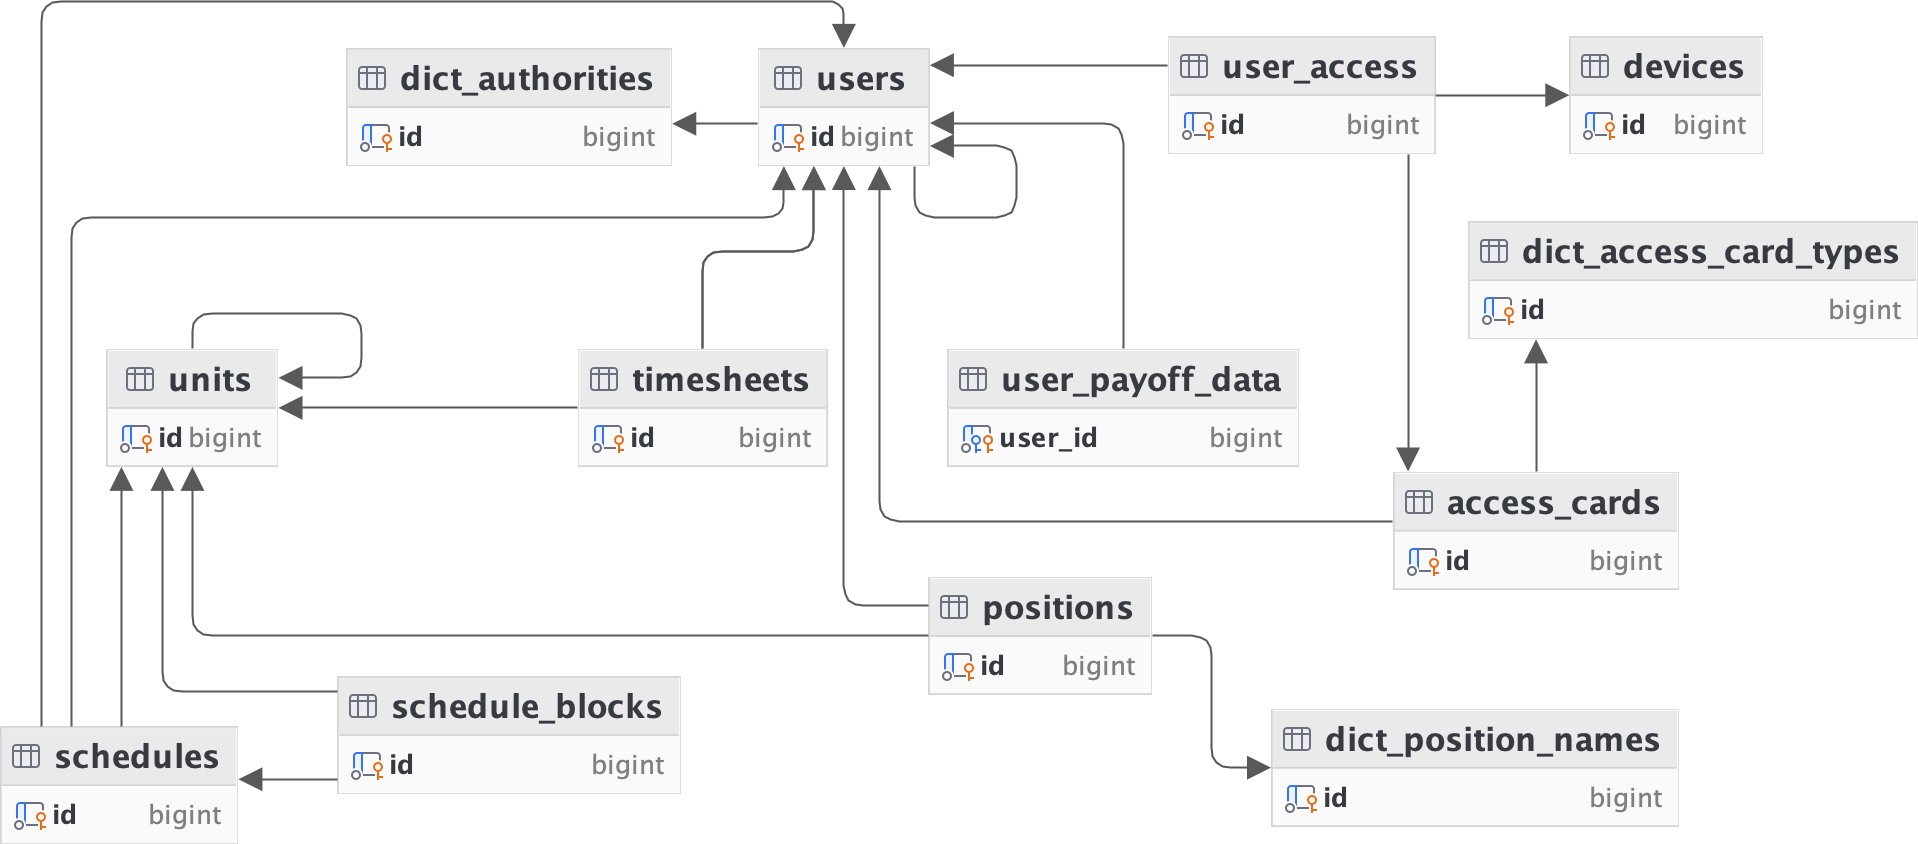
\includegraphics[width=\textwidth]{graf/dbDiagram.png}
    \caption{Uproszczony schemat bazy danych}
    \label{fig:dbDiagram}
\end{figure}

\subsection{Tabele użytkowników}

\begin{figure}[H]
    \centering
    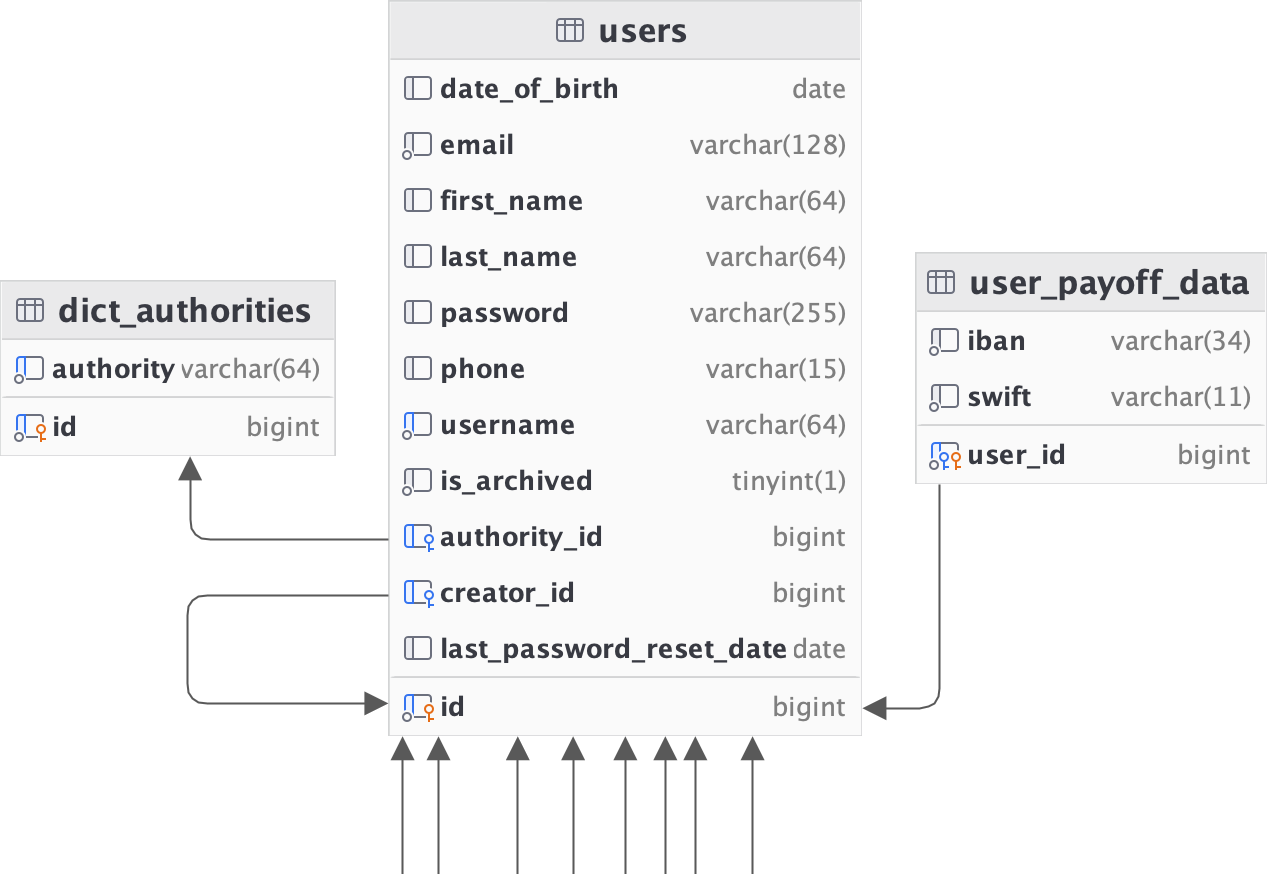
\includegraphics[width=0.7\textwidth]{graf/usersTable.png}
    \caption{Schemat tabel użytkowników}
    \label{fig:usersTable}
\end{figure}

Główną tabelą przechowującą informacje o użytkownikach jest tabela \texttt{USERS}. Zawiera ona dane personalne, takie jak imię, nazwisko, adres e-mail i numer telefonu. Dodatkowo do tabeli wpisane są dane do logowania: nazwa użytkownika i hasło; oraz informacja o użytkowniku, który  utworzył dany wpis. Każdy użytkownik ma przypisaną jedną z ról z tabeli \texttt{DICT\_AUTHORITIES}, która określa jego uprawnienia w systemie - w relacji wiele do jednego. Relacją jeden do jednego jest połączona tabela \texttt{USER\_PAYOFF\_DATA} zawierające dane o koncie bankowym użytkownika. W tabeli \texttt{USERS} znajduje się również pole \texttt{is\_archived}, które określa, czy użytkownik jest aktywny w systemie.

\subsection{Tabele jednostek organizacyjnych}

\begin{figure}[H]
    \centering
    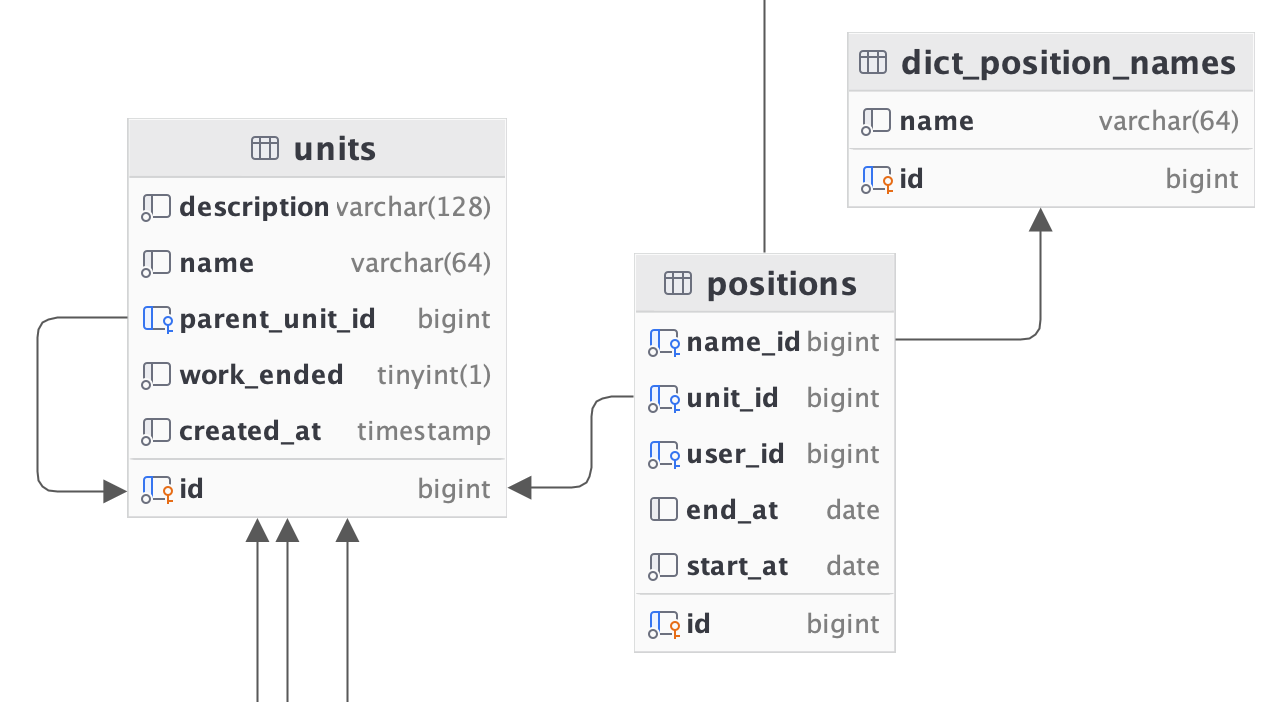
\includegraphics[width=0.8\textwidth]{graf/unitsTable.png}
    \caption{Schemat tabel jednostek organizacyjnych}
    \label{fig:organizationalUnitsTable}
\end{figure}

Wszystkie jednostki organizacyjne są przechowywane w tabeli \texttt{UNITS} zawierającej dane o nazwie jednostki, jej opisie, jednostce nadrzędnej oraz dacie utworzenia. Pole \texttt{work\_ended} określa, czy jednostka jest aktywna. Użytkownicy są przypisani do jednostki organizacyjnej poprzez tabelę \texttt{positions} będącą tabelą łącznikową między tabelami \texttt{USERS} i \texttt{UNITS}. Znajdują się w niej dane o dacie rozpoczęcia pracy na danym stanowisku oraz dacie zakończenia pracy, a także odwołanie do tabeli słownikowej, zawierającej nazwy stanowisk. Tabela \texttt{POSITIONS} jest szczególnie ważna przy odczytywaniu harmonogramów pracy.

\subsection{Tabele harmonogramów}

\begin{figure}[H]
    \centering
    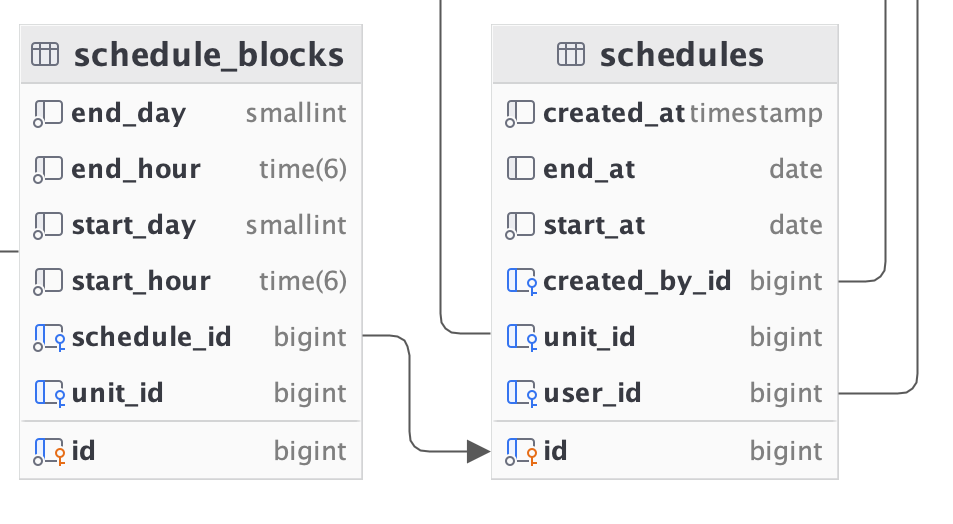
\includegraphics[width=0.7\textwidth]{graf/scheduleTable.png}
    \caption{Schemat tabel harmonogramów}
    \label{fig:schedulesTable}
\end{figure}

Na każdy z harmonogramów składa się pojedynczy rekord w tabeli \texttt{SCHEDULES} oraz pewna liczba rekordów w tabeli \texttt{SCHEDULE\_BLOCKS}. Pierwsza z nich zawiera informacje o dacie rozpoczęcia i zakończenia harmonogramu, jego utworzenia oraz odwołanie do jednostki organizacyjnej lub użytkownika, którego dotyczy. Tabela \texttt{SCHEDULE\_BLOCKS} odpowiada za przechowywanie pojedynczych bloków czasowych w harmonogramie opisując ich dzień i godzinę rozpoczęcia oraz zakończenia oraz jednostkę, której dotyczą. Tabele są powiazane relacją jeden do wielu - jeden harmonogram może zawierać wiele bloków czasowych.

\subsection{Tabele kart dostępowych}

\begin{figure}[H]
    \centering
    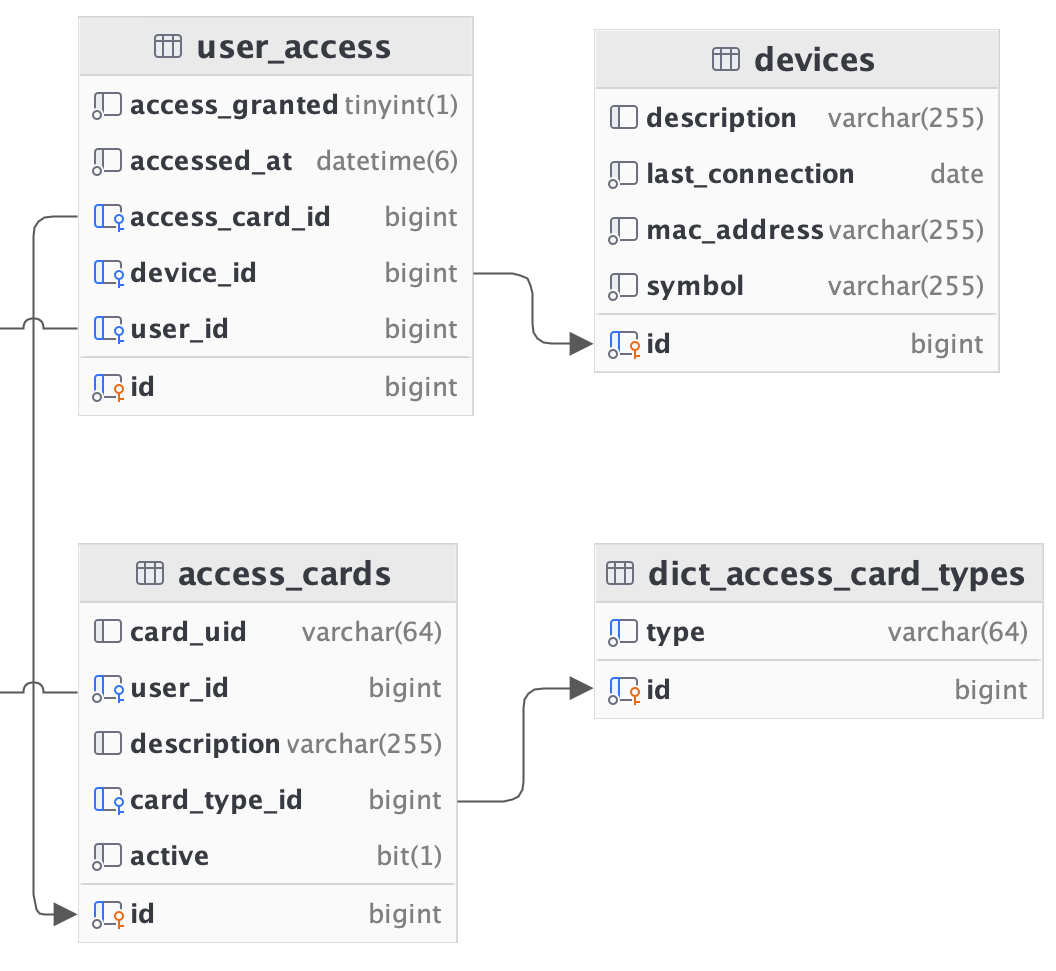
\includegraphics[width=0.7\textwidth]{graf/acTable.png}
    \caption{Schemat tabel kart dostępowych}
    \label{fig:accessCardsTable}
\end{figure}

Karty dostępowe użytkowników są przechowywane w tabeli \texttt{ACCESS\_CARDS} zawierającej informacje o numerze seryjnym, jej właścicielu opisie, typie karty oraz statusie. Dzięki ostatniej z właściwości możliwe jest przypisanie dwóm użytkownikom jednej karty w różnych okresach czasu. Każda autoryzacja użytkownika jest zapisywana w tabeli \texttt{USER\_ACCESS} wpisując do niej datę i godzinę, id użytkownika, id czytnika, id karty dostępowej oraz status autoryzacji. Umożliwia to późniejsze analizowanie historii autoryzacji.

Tabela \texttt{DEVICES} przechowuje informacje o czytnikach kart - ich opis, datę ostatniego uruchomienia, adres MAC (ang. \english{Media Access Control address}) oraz symbol, którym identyfikuje się w systemie.

\subsection{Tabele słownikowe}

W bazie danych znajdują się trzy tabele słownikowe zawierające dane, które nie zmieniają się w czasie działania systemu. Każda z nich poprzedzona jest prefiksem \texttt{DICT\_}. Są to:

\begin{itemize}
    \item \texttt{DICT\_AUTHORITIES} zawierająca role użytkowników, równoznaczne z uprawnieniami,
    \item \texttt{DICT\_ACCESS\_CARD\_TYPES} zawierająca typy kart dostępowych dla łatwiejszego rozróżnienia tagów NFC,
    \item \texttt{DICT\_POSITION\_NAMES} zawierająca nazwy stanowisk przypisanych pracownikom.
\end{itemize}

Do tabel \texttt{DICT\_ACCESS\_CARD\_TYPES} i \texttt{DICT\_POSITION\_NAMES} mogą zostać dodane nowe rekordy, lecz nie jest możliwe ich usunięcie. Takie ograniczenie zapewnia integralność danych w systemie i zapobiega błędom w działaniu aplikacji.

Dane mogą dodawać jedynie administratorzy systemu.

\section{Modele i struktury danych}

\note{W tej części pracy należy opisać, jakie modele danych zostały zastosowane w systemie. Należy zaznaczyć, jakie są relacje między nimi.}

\subsection{Model użytkownika}

\section{Algorytmy}

\subsection{Rejestracja i pierwsze logowanie użytkownika}

Rejestracja użytkownika może zostać dokonana jedynie przez administratora systemu. W tym celu powinien on wypełnić formularz rejestracyjny wprowadzając nazwę użytkownika oraz jego adres email. Po zatwierdzeniu formularza, w widoku wszystkich użytkowników pojawi się nowy rekord z danymi właśnie utworzonego użytkownika. Następnie administrator powinien przekazać nowo zarejestrowanemu użytkownikowi jego nazwę, którą musi wpisać na ekranie logowania - nie jest wymagane przy tym wpisywanie hasła. Po zatwierdzeniu formularza, i wysłaniu danych do serwera, sprawdzi on czy użytkownik o podanej nazwie istnieje w bazie danych i czy ma przypisane hasło. Jeżeli nie, zwróci kod 206 - \texttt{Partial Content}, a aplikacja udostępni użytkownikowi możliwość ustawienia hasła. Po jego wpisaniu, potwierdzeniu i zatwierdzeniu formularza, użytkownik zostanie zalogowany do systemu. Diagram sekwencji pierwszego logowania użytkownika został przedstawiony na rysunku \ref{fig:login}, a szczegóły tego procesu zostały opisane w rozdziale \ref{ss:logowanie}

\subsection{Logowanie}
\label{ss:logowanie}

Logowanie do systemu odbywa się poprzez przesłanie żądania HTTP z danymi logowania do serwera aplikacyjnego. Po jego otrzymaniu serwer zwraca się do bazy danych w celu znalezienia użytkownika o podanej nazwie. Jeżeli użytkownik nie istnieje, serwer zwraca kod błędu 401. W przeciwnym wypadku sprawdza, czy zahashowane hasło użytkownika jest zgodne z zapisanym w bazie. Jeżeli hasła się zgadzają, serwer generuje dwa tokeny JWT (ang. \english{JSON Web Token}) i zwraca je w odpowiedzi. Aplikacja kliencka zapisuje otrzymane tokeny w pamięci lokalnej przeglądarki i przechodzi do widoku panelu głównego. Diagram czynności logowania został przedstawiony na rysunku \ref{fig:login}.

\begin{figure}[H]
    \centering
    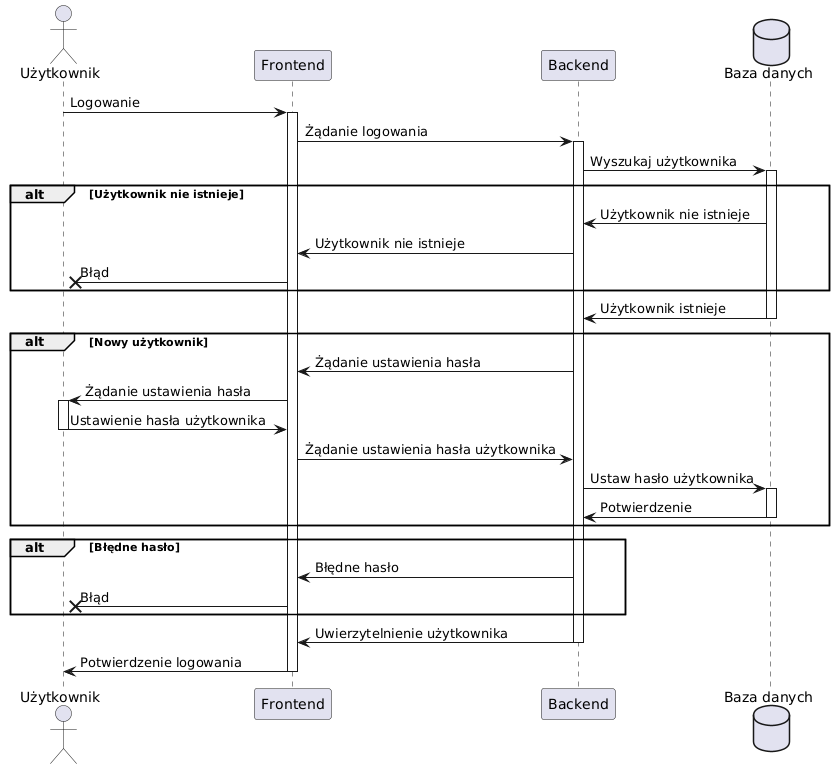
\includegraphics[width=0.9\textwidth]{graf/loginSequence.png}
    \caption{Diagram czynności logowania}
    \label{fig:login}
\end{figure}
% //www.pantum.com/plantuml/png/VP8nRiCm34LtdKB8dWju288CdOgYIz2PigX6iIC5jbJN7WFq43rBEzRtAeceK6pKcJpyh__9Hs_R04s8frf06NmZz-Dt7ohVELj9QAMBuaowBUqPN90FZNS1dMR9u4JQGLabHQ7G4411YtArWm6a1jUNXnMBMWaXN9Jh3IN8GZxwLz-1iyW3s3S8oCa6rnl5ylZryw5PbdKoGZPIaK9EqegiBtqxn0gECkOTifcBeGwJ1JdMje4-HnfPSHANBdfIcxdhCUnv9t9aseqN6byG5uhdZMOFSpdEvtpoNN-xYL24n4oHH3fUPv6Oo0EqumK4StFnhYaZuUkwoAd5_i-4oJI5gF7cJJfEiLmnUysJQqMRi-tgy8j7Ig0A-Um3PJPweDmv80RAa9ZlftQOGZEZkM3mdvja-vwRXZvWxQuGbhPNwRuSDHin_w2t3moABLN5K_qB

\subsection{Uwierzytelnianie użytkownika}

Klient po zalogowaniu się do systemu otrzymuje od serwera dwa tokeny JWT, które są przechowywane w pamięci lokalnej przeglądarki. Aby mógł korzystać z zasobów serwera, musi dołączać pierwszy z nich - token dostępowy - do nagłówka każdego żądania HTTP pod kluczem \texttt{Authorization} poprzedzając go słowem \texttt{Bearer}. Przykładowy nagłówek został przedstawiony na rysunku. Token ten jest ważny przez określony czas, po którym traci ważność - serwer zwraca wtedy kod błędu 401. Jeżeli zaistnieje taka sytuacja, klient musi wysłać żądanie odświeżenia tokena do serwera, dołączając drugi token - odświeżający - który ma dłuższy czas przedawnienia. Serwer następnie sprawdza, czy token odświeżający jest poprawny i zwraca nowe tokeny. W przeciwnym wypadku klient musi ponownie zalogować się do systemu. Diagram sekwencji procesu uwierzytelniania użytkownika został przedstawiony na rysunku \ref{fig:authSequence}.

\begin{figure} [H]
    \centering
    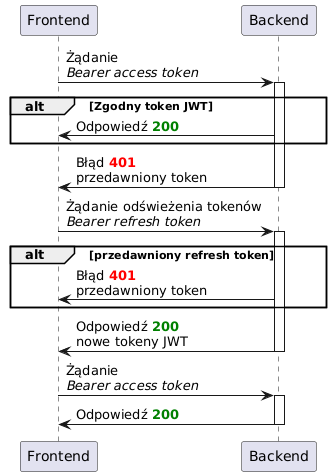
\includegraphics[width=0.4\textwidth]{graf/jwtSeq.png}
    \caption{Diagram sekwencji procesu uwierzytelniania użytkownika}
    \label{fig:authSequence}
\end{figure}
% //www.plantuml.com/plantuml/png/fPAnIiH048RxVOhX-a0KAudBaSB2naOG9CraPt8knjcmMGrdAVWKFeQTscdUopLHk1K5zQeKy__pV_zabtr07wukMzN5hpMsGmbmw9q45WBieU5aLAAv-9ZKh5J3cQuPzc5yUhqZ5CjGIM5roUZP0nh3VG_1HOz24-mr1dutOXlWREL8rlCGZavFL5oKwHWOrnrJvmRBD3v2qKGOCAvr_c2nyiooq4MjT_DSiL0qPNgobEDjH4ZbdcaIx-KxbNJ-XWa7iUupLH5lG7rNnj5u7pd6PnQBi-dbOTYiwBdnt9__q379JANRW2VDVtUiIiGDFDlNqxcJyl_-at-Z-1Agr9A5ulDx0m00

\subsection{Harmonogramowanie}

\subsection{Przypisanie  karty dostępowej}

Przypisanie karty dostępowej odbywa się przy wykorzystaniu aplikacji mobilnej. Po zalogowaniu się do systemu administrator powinien wybrać zakładkę \texttt{CARDS}, a następnie rozpocząć skanowanie tagu NFC. Po pozytywnym odczytaniu danych aplikacja wyśle do serwera żądanie o informacje na temat karty, a w kolejnym kroku wyświetli informacje jej właścicielu. Jeżeli karta jest już przypisana do użytkownika, aplikacja umożliwi jej usunięcie, a w przeciwnym wypadku udostępni menu wyboru użytkownika, do którego ma zostać przypisana. Po zatwierdzeniu wyboru, aplikacja wyśle do serwera żądanie przypisania karty do użytkownika. Diagram sekwencji przypisania karty dostępowej został przedstawiony na rysunku \ref{fig:assignCard}.


\begin{figure}[H]
    \centering
    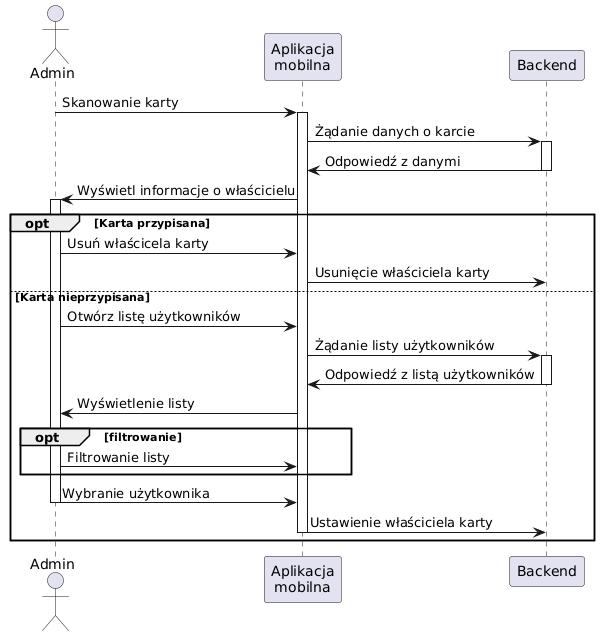
\includegraphics[width=0.7\textwidth]{graf/cardSeq.png}
    \caption{Diagram sekwencji odczytu i przypisania karty dostępowej}
    \label{fig:assignCard}
\end{figure}
% //www.plantuml.com/plantuml/png/TP8nKiCm44LxdM8dVIv0aKaeQ2XIC0mDpThQ38jbIMFBU9oI8OV8v1ZfW2xnlTW8W-r0YgY8tlx_zylpCc0HgjmeJ8ChOA5pje0be5PURZXbZpR0PE4DPvW-uwFDNSB6uYHYte-uQqmpilfqbP1IgASpGU0AxZAqhaRB19dmpScFNp1Gb93VT9QGSEt7SQCZ9cUJFe4xyIbJFo32WavdyAsyrDxLJBfzXtKSobbf6j9H7RMm3qsx4pOOOBjoHIuBaJZKxIkskvJ5nbI3P5ev7-1MyYBuOjruBj6Y0kZtkY-hzgqN88FTVW3zKW9PFcv5Vc3LesHAwbnayGj6or0VziKQ39VXk8Mg_Mn2vchBsM5V2_bFXP5jpj5nZr5-t6BdiJaR_5jgV8DHhVJh6fjRiGb5V7NXTVzaD_t_7KrM3mbHJ8fuFSY0mmIeVn9q3GUK1FP2myD1xwERciif7_uN

\section{Użyte biblioteki i frameworki}

\note{Ta część może się znaleźć przy przeglądzie technologii.} % [Właściwy dla kierunku -- np. Specyfikacja wewnętrzna]

% TODO
\chapter{Weryfikacja i walidacja}
\label{ch:06}
% \begin{itemize}
% \item sposób testowania w ramach pracy (np. odniesienie do modelu V)
% \item organizacja eksperymentów
% \item przypadki testowe zakres testowania (pełny/niepełny)
% \item wykryte i usunięte błędy
% \item opcjonalnie wyniki badań eksperymentalnych
% \end{itemize}

% \begin{table}
% \centering
% \caption{Nagłówek tabeli jest nad tabelą.}
% \label{id:tab:wyniki}
% \begin{tabular}{rrrrrrrr}
% \toprule
% 	         &                                     \multicolumn{7}{c}{metoda}                                      \\
% 	         \cmidrule{2-8}
% 	         &         &         &        \multicolumn{3}{c}{alg. 3}        & \multicolumn{2}{c}{alg. 4, $\gamma = 2$} \\
% 	         \cmidrule(r){4-6}\cmidrule(r){7-8}
% 	$\zeta$ &     alg. 1 &   alg. 2 & $\alpha= 1.5$ & $\alpha= 2$ & $\alpha= 3$ &   $\beta = 0.1$  &   $\beta = -0.1$ \\
% \midrule
% 	       0 &  8.3250 & 1.45305 &       7.5791 &    14.8517 &    20.0028 & 1.16396 &                       1.1365 \\
% 	       5 &  0.6111 & 2.27126 &       6.9952 &    13.8560 &    18.6064 & 1.18659 &                       1.1630 \\
% 	      10 & 11.6126 & 2.69218 &       6.2520 &    12.5202 &    16.8278 & 1.23180 &                       1.2045 \\
% 	      15 &  0.5665 & 2.95046 &       5.7753 &    11.4588 &    15.4837 & 1.25131 &                       1.2614 \\
% 	      20 & 15.8728 & 3.07225 &       5.3071 &    10.3935 &    13.8738 & 1.25307 &                       1.2217 \\
% 	      25 &  0.9791 & 3.19034 &       5.4575 &     9.9533 &    13.0721 & 1.27104 &                       1.2640 \\
% 	      30 &  2.0228 & 3.27474 &       5.7461 &     9.7164 &    12.2637 & 1.33404 &                       1.3209 \\
% 	      35 & 13.4210 & 3.36086 &       6.6735 &    10.0442 &    12.0270 & 1.35385 &                       1.3059 \\
% 	      40 & 13.2226 & 3.36420 &       7.7248 &    10.4495 &    12.0379 & 1.34919 &                       1.2768 \\
% 	      45 & 12.8445 & 3.47436 &       8.5539 &    10.8552 &    12.2773 & 1.42303 &                       1.4362 \\
% 	      50 & 12.9245 & 3.58228 &       9.2702 &    11.2183 &    12.3990 & 1.40922 &                       1.3724 \\
% \bottomrule
% \end{tabular}
% \end{table}  

 % Weryfikacja i walidacja

% TODO
\chapter{Podsumowanie i wnioski}

\section{Wnioski}

Celem pracy było zaprojektowanie i implementacja systemu do zarządzania personelem w firmie. Umożliwia on zarządzanie pracownikami, ich zadaniami, czasem pracy i strukturą firmy w sposób zautomatyzowany. Wymierne korzyści z zastosowania systemu to zwiększenie efektywności pracy, zwiększenie kontroli nad zadaniami i pracownikami oraz zwiększenie przejrzystości ról w firmie. Przeprowadzona analiza wymagań pozwoliła na stworzenie systemu, który spełnia oczekiwania użytkowników, co potwierdziły przeprowadzone testy.

Wynikiem pracy jest system, który spełnia założenia projektowe i udostępnia użytkownikom sprecyzowane w wymaganiach funkcjonalności. Jest on bezpieczny, łatwy w obsłudze i automatyzuje szereg procesów, które wcześniej były wykonywane ręcznie. Aplikacja mobilna pozwala na dostęp do systemu z każdego miejsca i w każdym czasie, a dzięki funkcji dodawania kart zbliżeniowych niweluje konieczność ręcznego wpisywania danych lub użycia czytników podłączanych do komputera. Użycie mikrokontrolerów pozwala na automatyzację zapisu czasu pracy pracowników, co znacznie ułatwia jego śledzenie. Dzięki ich zastosowaniu możliwa jest również obsługa kontroli dostępu do pomieszczeń.

System został zrealizowany w wersji podstawowej, jednak posiada wiele możliwości rozwoju. Udało się zrealizować funkcjonalności dotyczące: rejestracji czasu pracy, zarządzania pracownikami, harmonogramami pracy, zadaniami, czasem pracy i strukturą firmy. Nie udało się zrealizować funkcjonalności dotyczących raportów, wniosków oraz automatycznego śledzenia czasu pracy pracowników. Wszystkie one mogą jednak zostać dodane w przyszłości, co znacznie zwiększyłoby użyteczność systemu. Implementacja kontroli dostępu do pomieszczeń została zrealizowana w ograniczonym zakresie, jednak możliwe jest jej rozbudowanie.

\subsection{Problemy napotkane podczas pracy}

Podczas pracy napotkano kilka problemów, które znacząco ją utrudniły i wydłużyły. Największym problemem było to, że przy projektowaniu systemu nie wzięto pod uwagę stopnia jego złożoności. Poskutkowało to koniecznością zrezygnowania z części funkcjonalności lub ograniczeniem ich zakresu na rzecz dotrzymania terminu.

W założeniach aplikacji mobilnej, miała ona umożliwiać autoryzację użytkownika poprzez przyłożenie urządzenia do czytnika kart zbliżeniowych. Niestety, przez decyzje podjęte na etapie projektowania komunikacji między układem mikrokontrolera a serwerem, nie udało się zrealizować tej funkcjonalności. Autoryzacja opiera się o numery seryjne kart, co znacznie ułatwia proces ich odczytania i rejestracji. Urządzenie mobilne musiało by być w stanie emulować te numery, jednakże nie jest to możliwe bez modyfikacji systemu operacyjnego.

Framework \texttt{Expo} użyty do stworzenia aplikacji mobilnej udostępniał funkcję odczytywania zmiennych środowiskowych. Niestety, po pewnym czasie funkcja przestała odświeżać wartości, co wiązało się z koniecznością częstej, wielokrotnej kompilacji aplikacji. Problem ten nie został rozwiązany, co znacznie wydłużyło pracę nad aplikacją mobilną.

\subsection{Ocena dobranych technologii po zakończeniu pracy}

Technologie wybrane do realizacji systemu okazały się być idealne, ponieważ w sposób znaczący przyspieszyły pracę nad projektem. Mikrokontroler, na którym zainstalowano system \texttt{MicroPython} okazał się być bardo prosty w obsłudze i umożliwił szybkie zaimplementowanie funkcjonalności związanych z odczytem kart zbliżeniowych. \texttt{Spring Framework} nie sprawił, że system stał się zbyt skomplikowany, a wręcz przeciwnie - pozwolił na jasne zdefiniowanie struktury aplikacji i łatwe zarządzanie nią. Framework \texttt{Vue.js} zrobił na autorze bardzo dobre wrażenie swoją prostotą i intuicyjnością. W porównaniu z innymi frameworkami, takimi jak \texttt{Next.js}, okazał się być znacznie przyjaźniejszy, jawnie oddzielając warstwę prezentacji, logiki i danych. \texttt{Expo} okazało się najbardziej uciążliwą technologią, jednakże poza wymienionym nie sprawiło innych problemów. Użycie innej technologii, np. \texttt{Flutter} mogłoby przyspieszyć pracę nad aplikacją mobilną, jednakże konieczność nauki nowego frameworka mogłaby wydłużyć czas potrzebny na jej stworzenie.

\section{Perspektywy rozwoju}

System posiada wiele możliwości rozwoju, które znacznie zwiększyłyby jego użyteczność. Pierwszym krokiem, jaki należy podjąć jest zwiększenie ilości czytników kart zbliżeniowych - obecnie w systemie działa tylko jeden, ale możliwe jest łatwe podłączenie większej ich ilości. Następnie należałoby zająć się brakującymi częściami: raportami, wnioskami i automatycznym śledzeniem czasu pracy pracowników. Raporty powinny być generowane w formie plików PDF (ang. \english{Portable Document Format}), które można by było wydrukować lub przesłać mailem. Do wniosków - oprócz możliwości ich składania i akceptacji - dobrze byłoby dodać możliwość wymieniania się wiadomościami w formie czatu. Automatyczne śledzenie czasu pracy może być zrealizowane algorytmicznie, wywołując odpowiednie funkcje w określonych momentach. Możliwe, że dobrym wyborem było by zastosowanie algorytmów uczenia maszynowego, które nauczyły by się rozpoznawać co pracownik robi w danym momencie. Kontrola dostępu do pomieszczeń również wymaga rozbudowy - aktualnie użytkownicy mogą autoryzować się przy każdym czytniku bez ustalania dostępu do pomieszczeń. W przyszłości warto byłoby dodać możliwość ustalania uprawnień dla poszczególnych użytkowników. W dalszej perspektywie można rozszerzać system o kolejne funkcjonalności znane z systemów HCM.

\section{Podsumowanie}

Samodzielne stworzenie systemu, który spełnia podane wymagania, jest bardzo czasochłonne. Wymaga od programisty bardzo dużej wiedzy, umiejętności i zaangażowania. Duże zespoły są w stanie tworzyć systemy o wiele bardziej rozbudowane i złożone w krótszym czasie - co widać po rozwiązaniach dostępnych na rynku. Każdy z członków zespołu wnosi do projektu swoje doświadczenie, wiedzę i specjalizację, dzięki czemu praca nad projektem jest bardziej efektywna i przyjemna.

Wykonanie projektu pozwoliło na zrozumienie procesów zachodzących w firmach i ukazało, jakie korzyści przynosi zastosowanie systemu informatycznego. Praca nad systemem pozwoliła na zdobycie ogromnych zasobów wiedzy - tak technicznej, jak i biznesowej. Projekt okazał się być dużym wyzwaniem, ale również przyniósł wiele satysfakcji. Udało się stworzyć system, który spełnia założenia projektowe i jest gotowy do dalszego rozwoju. Praca nad projektem pozwoliła na zdobycie cennego doświadczenia i wiedzy, które przyniosą wymierne korzyści w przyszłości. System posiada wiele możliwości rozwoju, które mogą znacznie zwiększyć jego użyteczność i funkcjonalność. Warto kontynuować prace nad nim, aby w pełni wykorzystać jego potencjał. % Podsumowanie i wnioski

\backmatter

%\bibliographystyle{plplain}  % bibtex
%\bibliography{biblio/biblio} % bibtex
\printbibliography           % biblatex
\addcontentsline{toc}{chapter}{Bibliografia}

\begin{appendices}

% TODO
\chapter{Spis skrótów i symboli}

\begin{itemize}
    % \item[DNA] kwas deoksyrybonukleinowy (ang. \english{deoxyribonucleic acid})
    % \item[MVC] model -- widok -- kontroler (ang. \english{model--view--controller}) 
    % \item[$N$] liczebność zbioru danych
    % \item[$\mu$] stopnień przyleżności do zbioru
    % \item[$\mathbb{E}$] zbiór krawędzi grafu
    % \item[$\mathcal{L}$] transformata Laplace'a 
    \item[HCM] System Zarządzania Kapitałem Ludzkim (ang. \english{Human Capital Management})
    \item[HR] Zarządzanie Zasobami Ludzkimi (ang. \english{Human Resources})
    \item[CRM] Zarządzanie Relacjami z Klientami (ang. \english{Customer Relationship Management})
    \item[SPA] Aplikacja jednostronicowa (ang. \english{Single Page Application})
    \item[MAC] Adres sprzętowy karty sieciowej (ang. \english{Media Access Control address})
    \item[DTO] Obiekt transferu danych (ang. \english{Data Transfer Object})
    \item[MSC] Model-Serwis-Kontroler (ang. \english{Model-Service-Controller})
    \item[EAS] Usługa aplikacji Expo (ang. \english{Expo Application Services})
\end{itemize}
 % Spis skrótów i symboli

% TODO
\chapter{Źródła}

Jeżeli w pracy konieczne jest umieszczenie długich fragmentów kodu źródłowego, należy je przenieść w to miejsce.

\begin{lstlisting}
if (_nClusters < 1)
	throw std::string ("unknown number of clusters");
if (_nIterations < 1 and _epsilon < 0)
	throw std::string ("You should set a maximal number of iteration or minimal difference -- epsilon.");
if (_nIterations > 0 and _epsilon > 0)
	throw std::string ("Both number of iterations and minimal epsilon set -- you should set either number of iterations or minimal epsilon.");
\end{lstlisting}


% % % % % % % % % % % % % % % % % % % % % % % % % % % % % % % % % % % 
% Pakiet minted wymaga odkomentowania w pliku config/settings.tex   %
% importu pakietu minted: \usepackage{minted}                       %
% i specjalnego kompilowania:                                       %
% pdflatex -shell-escape praca                                      %
% % % % % % % % % % % % % % % % % % % % % % % % % % % % % % % % % % % 

\begin{minted}[linenos,breaklines,frame=lines]{c++}
if (_nClusters < 1)
  throw std::string ("unknown number of clusters");
if (_nIterations < 1 and _epsilon < 0)
  throw std::string ("You should set a maximal number of iteration or minimal difference -- epsilon.");
if (_nIterations > 0 and _epsilon > 0)
  throw std::string ("Both number of iterations and minimal epsilon set -- you should set either number of iterations or minimal epsilon.");
\end{minted}
 % Źródła

% TODO
\chapter{Lista dodatkowych plików, uzupełniających tekst pracy} 


% W systemie do pracy dołączono dodatkowe pliki zawierające:
% \begin{itemize}
% \item źródła programu,
% \item dane testowe,
% \item film pokazujący działanie opracowanego oprogramowania lub zaprojektowanego i~wykonanego urządzenia,
% \item itp.
% \end{itemize}
 % Lista dodatkowych plików, uzupełniających tekst pracy

\listoffigures
\addcontentsline{toc}{chapter}{Spis rysunków}
\listoftables
\addcontentsline{toc}{chapter}{Spis tabel}

\end{appendices}

\end{document}


%% Finis coronat opus.

